\documentclass[english]{article}

\title{\vspace{-5.5ex} \bf Design Project 3: Dynamic Scheduling}
\author{{\bf Connor Smith} \\
	{\small Department of Electrical and Computer Engineering} \\
	{\small Brigham Young University, Provo, UT 84602} \\
	{\small connor.smith.256@gmail.com} \\
}

\usepackage{babel}
\usepackage[margin=1in]{geometry}
\usepackage{hyperref}
\usepackage{graphicx}
\usepackage{float}
\usepackage{caption}
\usepackage{subcaption}
\usepackage{setspace}

\date{\today}

\begin{document}
\doublespacing
\maketitle

\section{Introduction}
For decades, processors have used pipelining to exploit instruction-level parallelism. However, dependences among instructions as well as memory latency result in pipeline stalls and reduce throughput. Out-of-order processors seek to minimize the number of idle cycles by reordering the execution of instructions, a process known as dynamic scheduling. As long as this reordering is guaranteed to produce the same results as in-order execution, dynamic scheduling can minimize or hide stalls, increasing overall performance.

Many architectural parameters contribute to the organization of a processor. For a typical processor, these include the cache configuration, branch predictor, and number of functional units. For out-of-order processors, these also include the instruction queue size, the decode bandwidth, the RUU issue width and size, instruction commit bandwidth, and the load/store queue size. Each of these (and others) must be carefully chosen to maximize the desired characteristics. Since the design space is so large, it is necessary to use a methodology that is capable of considerably narrowing the space to determine the best configuration for a chosen market.

\section{Design Methodology}

\subsection{Base Configuration}
The design choices in this project reflect the target market of mid- to high-performance desktop computing. As a result, the primary characteristic of concern is overall performance. Since the cycle time is set to 600 MHz and does not vary from one design to the next, instructions per cycle (IPC) is a fair metric to use when comparing the performance of different configurations. Constraints were also placed on the average and maximum power consumption of the processor in an attempt to limit designs to those applicable to a typical desktop computer that does not require any special cooling.

The starting configuration is mostly based off of the default values in sim-outorder, with some modifications. The L1 and L2 cache configurations are based off those used in Intel's Haswell architecture and used in Design Project 1, and these remain constant across all designs explored in this project, since the focus of this project is on dynamic scheduling. The memory latency was fixed at 100ns, which corresponds to 60 cycles for a processory running at 600 MHz. Also, a perfect branch predictor was chosen for all of the designs. It should be noted that this limits the accuracy of the results; the reported IPC will be higher than in reality, and the reported power will likely be slightly lower. However, this choice eliminates a source of complexity, and the ranking of which designs are better should remain roughly the same. In addition, it is unlikely that the architecture would be utilized to its full potential when using an imperfect predictor, so the use of a perfect branch predictor should illustrate the full difference in performance between designs. Thus the end goal is less focused on presenting completely accurate metrics for a given design and more on determining which designs are better relative to  others. The parameters related to out-of-order execution in the starting configuration were set to be the defaults of sim-outorder. Table 1 shows a summary of the base configuration.

\begin{center}
    \singlespacing
	\captionof{table}{Baseline configuration}
	\vspace{.30cm}
	\begin{tabular}{ | l | l | l | l | l | l |}
	\hline
      L1 Capacity & 32KB \\ \hline
      L1 Associativity & 8 \\ \hline
      L2 Capacity & 128KB \\ \hline
      L2 Associativity & 8 \\ \hline
      Block Size & 64 \\ \hline
      Memory latency & 60 \\ \hline
      Branch prediction & perfect \\ \hline
	  IFQ size & 4 \\ \hline
      Decode width & 4 \\ \hline
      Issue width & 4 \\ \hline
      Commit width & 4 \\ \hline
      RUU size & 16 \\ \hline
      LSQ size & 8 \\ \hline
      I ALU & 4 \\ \hline
      I MULT & 1 \\ \hline
      FP ALU & 4 \\ \hline
      FP MULT & 1 \\ \hline
	\end{tabular}
\end{center}

\subsection{Parameter Variation}
Efficient parameter variation is necessary to narrow the design space. For each configuration that is the best so far, a single next parameter is chosen and varied. If the new configuration is better overall, then the parameter is further varied in the same direction until it is no longer beneficial. At this point, a new parameter is chosen and the process repeats until no further optimizations can be made. It is important to note that parameter values for a local maxima are not necessarily the same as for global maxima. In other words, the "best" value for a given parameter may change after altering a different parameter. Because of this, parameters were revisited at the end of the analysis to ensure that the chosen design really is the best so far.

The most important criterion for whether a given configuration change is beneficial is raw performance, measured in IPC. For many changes, however, the IPC increases slightly but at the cost of significantly more power dissipation. This tradeoff is evaluated and a determination is made whether it is worth it. Since the target market for these designs is desktop computing, a soft power limit was set at 150W. Both average and maximum power per cycle are used in these considerations. Average power is important for overall energy consumption, while maximum power is an important consideration due to heat dissipation issues. SimpleScalar offers multiple different power models, and the non-ideal conditional clocking (CC3) model was used for this project.

There are a few more metrics that were used to determine which parameter to change next. These are the fractions of time that the instruction queue, register update unit, and load/store queues were full. While these statistics are not directly useful for determining which configuration is best, they do provide a guide for whether greater performance would result from changing the parameter that corresponds to the full rate for a given unit.

\section{Configurations and Results}
\subsection{Preliminary Configurations}
The results for the baseline configuration are shown in Figures 1 and 2. As can be seen, the IPC varies wildly from one benchmark to the next, ranging from 0.162 to 2.72, with a mean of 1.330. The SPEC benchmarks are quite diverse, so in order for a configuration to be better, it must yield an increase in the average IPC (and hopefully across all benchmarks).

\begin{figure}[H]
	\centering
	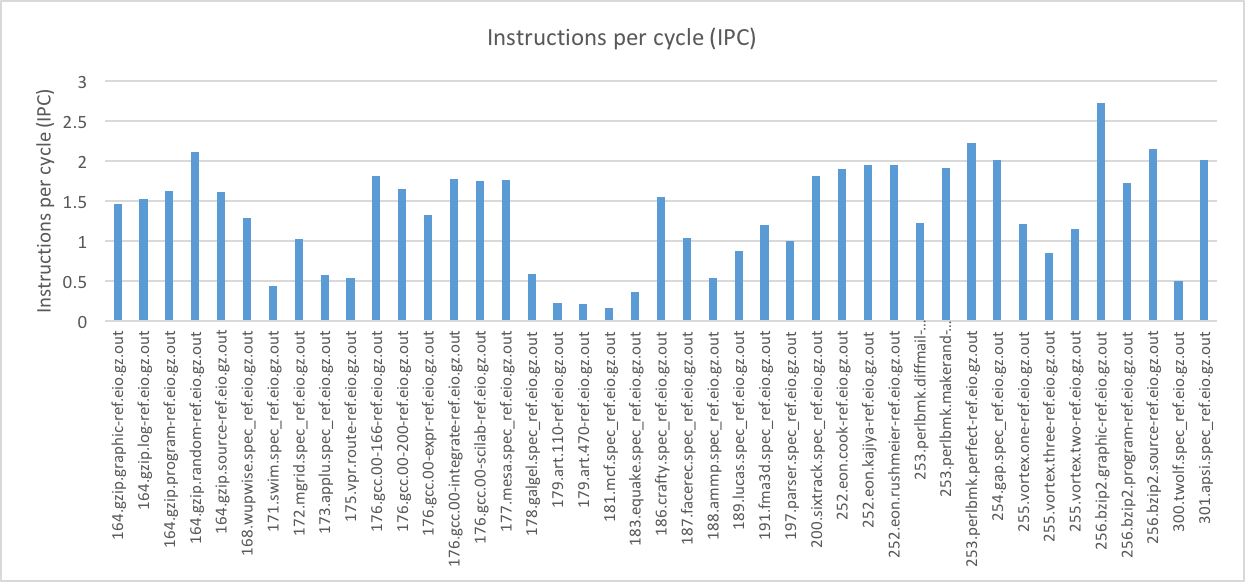
\includegraphics[height=8cm]{baseline_ipc.png}
	\caption{Instructions per cycle by benchmark}
\end{figure}

\begin{figure}[H]
	\centering
	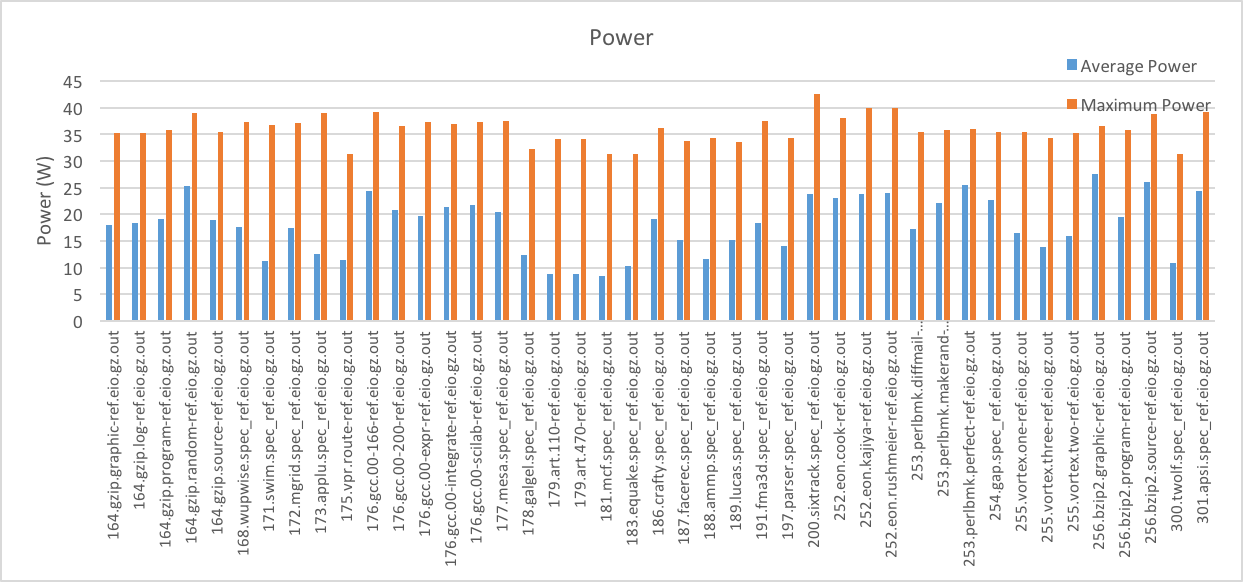
\includegraphics[height=8cm]{baseline_p.png}
	\caption{Average and maximum power by benchmark}
\end{figure}

Table 2 shows the average results for several different preliminary configurations, including the baseline. These configurations were analyzed to understand how much of an effect some of the parameters have on IPC and power. The "Double" configuration is the result of doubling each of the values, which yielded significant performance increases and kept power reasonable. "Max FUs" is the result of increasing the number of all the functional units to 8, which is the maximum value supported by SimpleScalar. Interestingly, this had a negligible effect on IPC but resulted in a spike in power, which illustrates that there are little to no structural hazards with the functional units in the baseline configuration. The "Min FUs" configuration corresponds to having only a single functional unit of each type. This caused a dramatic drop in performance, and was used to compute a soft minimum for IPC.

\begin{center}
	\captionof{table}{Preliminary Configuration Results}
	\vspace{.30cm}
	\begin{tabular}{ | l | l | l | l | l | l |}
		\hline
	  & Baseline & Double & Max FUs & Min FUs \\ \hline
      IPC & 1.330 & 1.896 & 1.367 & 0.788 \\ \hline
      Average Power & 18.078 & 31.540 & 22.185 & 12.290 \\ \hline
      Peak Power & 36.070 & 75.266 & 43.278 & 25.416 \\ \hline
	\end{tabular}
\end{center}

\subsection{Register Update Unit}
The first parameter that was changed was the register update unit (RUU), which is a combination of reservations stations and a reorder buffer (ROB). Based off the results of the baseline configuration, the RUU was full 50\% of the time. Increasing the bandwidth of the other units will not help much if the RUU is full, so the size was increased to 32 and 64. This decreased the full rate to roughly 1\%. The results for these configurations are shown in Table 3. IPC sees a modest improvement of 1.05x, while average and peak power increase by roughly 25\% each. There are clearly diminishing returns when increasing IPC.

\begin{center}
	\captionof{table}{Increasing RUU Size}
	\vspace{.30cm}
	\begin{tabular}{ | l | l | l | l | l | l |}
		\hline
	 RUU Size & 16 & 32 & 64 \\ \hline
     IPC & 1.330 & 1.386 & 1.389 \\ \hline
     Average Power & 18.078 & 20.384 & 22.561 \\ \hline
     Peak Power & 36.070 & 40.135 & 44.555 \\ \hline
	\end{tabular}
\end{center}

\subsection{Out-of-Order Bandwidth}
With a larger RUU, a good next choice of parameter to alter was the bandwidths of the out-of-order units: the fetch queue size, decode width, issue width, and commit width. These values were increased from 4 to 8. While they could be increased separately, it did not seem to make much sense to do so. Thus for the sake of simplicity each value was altered as a group. The results are shown in Table 4. As with increasing the RUU size, changing these parameters yielded a modest improvement of 1.05x to IPC. This time, however, average and peak power increased by 43\% and 78\%, respectively. These numbers are still well within the typical range for a desktop CPU, so the increase in IPC is worth it.

\begin{center}
	\captionof{table}{Increasing Out-of-order Unit Size/Bandwidth}
	\vspace{.30cm}
	\begin{tabular}{ | l | l | l | l | l | l |}
		\hline
	 Size/BW & 4 & 8 \\ \hline
     IPC & 1.389 & 1.463 \\ \hline
     Average Power & 22.561 & 26.045 \\ \hline
     Peak Power & 44.555 & 60.148 \\ \hline
	\end{tabular}
\end{center}

\subsection{Functional Units}
Using the architecture at this point, the processor can reorder and feed multiple instructions per cycle to the functional units, but there are still only a few FUs available. To reduce this congestion, the count of each functional unit was doubled, bringing the number of ALUs to 8 and multiply units to 2 for both integer and floating-point. Table 5 shows the results for this change. Yet again, this change resulted in a 1.05x boost in IPC. Average power increased by another 40\%, and peak power increased by 46\%. At this point, the power ceiling for desktop computing isn't too far off from the peak value of 88W reached by this new configuration.

\begin{center}
	\captionof{table}{Adding Functional Units}
	\vspace{.30cm}
	\begin{tabular}{ | l | l | l | l | l | l |}
		\hline
	 Number of FUs (ALU, MULT) & (4, 1) & (8, 2) \\ \hline
     IPC & 1.463 & 1.547 \\ \hline
     Average Power & 26.045 & 36.479 \\ \hline
     Peak Power & 60.148 & 87.705 \\ \hline
	\end{tabular}
\end{center}

\subsection{Load/Store Queue}
Thus far, not much has been done about latencies due to memory constraints. Indeed, at this point, the L/S queue is full 80\% of the time. Increasing the size of the load/store queue can help hide these limitations. The size of the queue was increased from 8 to 16, and the results are shown in Table 6. This caused the largest increase in IPC so far (1.36x). The increases in average and peak power (22\% and 40\%, respectively) were also some of the smallest of the changes so far. Increasing the size of the L/S queue was clearly a big win.

\begin{center}
	\captionof{table}{Adding Functional Units}
	\vspace{.30cm}
	\begin{tabular}{ | l | l | l | l | l | l |}
		\hline
	 L/S Queue Size & 8 & 16 & 32 & 64 \\ \hline
     IPC & 1.547 & 1.886 & 2.073 & 2.100\\ \hline
     Average Power & 36.479 & 40.853 & 43.485 & 44.376 \\ \hline
     Peak Power & 87.705 & 106.141 & 116.737 & 122.404 \\ \hline
	\end{tabular}
\end{center}

\subsection{Returning to Past Parameters}
At this point, there has been an overall IPC improvement of 1.58x, at the cost of a 2.45x increase in average power and 3.4x gain in peak power. With a peak power of over 120W, any further changes must have dramatic performance increases to justify increasing the power consumption any further. Since the number of ALUs was already at the maximum value that SimpleScalar supports, only the out-of-order width parameters and the RUU size were left to revisit. Table 7 shows the results of these changes. Increasing the RUU size does yield a performance increase, but at the cost of increasing the peak power consumption to a whopping 206W, which simply cannot be justified. In addition, increasing the issue/dispatch/commit widths again actually resulted in a net decrease in IPC while still increasing power consumption drastically.

\begin{center}
	\captionof{table}{Revisiting Past Parameters}
	\vspace{.30cm}
	\begin{tabular}{ | l | l | l | l | l | l |}
		\hline
	 & Best So Far & Increasing RUU Size & Increasing width  \\ \hline
     IPC & 2.100 & 2.373 & 2.065 \\ \hline
     Average Power & 44.376 & 61.814 & 63.878 \\ \hline
     Peak Power & 122.404& 206.089 & 185.695  \\ \hline
	\end{tabular}
\end{center}

\section{Conclusion}
The final configuration is shown in Table 8, and a comparison of IPC for each benchmark is shown in Figure 3. There is a clear and significant improvement in performance; no benchmark performs worse under the new configuration, and while some see only marginal benefit, those with high starting IPC see a dramatic improvement.

\begin{center}
    \singlespacing
	\captionof{table}{Baseline configuration}
	\vspace{.30cm}
	\begin{tabular}{ | l | l | l | l | l | l |}
	\hline
	  IFQ size & 8 \\ \hline
      Decode width & 8 \\ \hline
      Issue width & 8 \\ \hline
      Commit width & 8 \\ \hline
      RUU size & 64 \\ \hline
      LSQ size & 64 \\ \hline
      I ALU & 8 \\ \hline
      I MULT & 2 \\ \hline
      FP ALU & 8 \\ \hline
      FP MULT & 2 \\ \hline
	\end{tabular}
\end{center}

\begin{figure}[H]
	\centering
	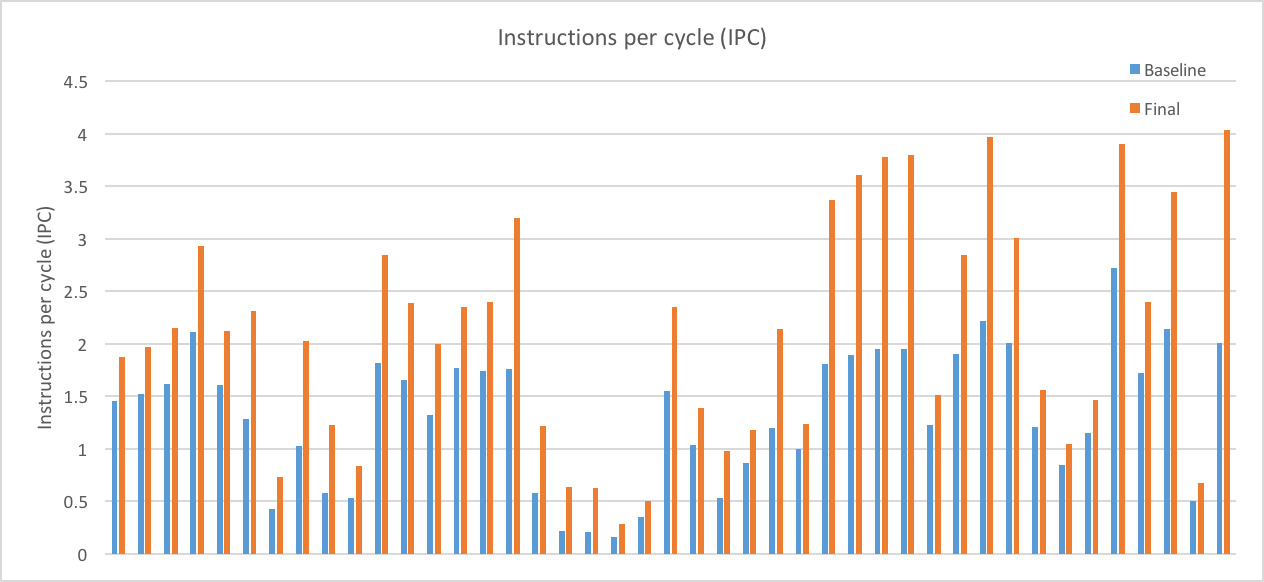
\includegraphics[height=8cm]{final.png}
	\caption{Baseline vs. Final configurations}
\end{figure}

Designing an out-of-order processor is clearly much more involved than designing a simple in-order one. Each of the different parameters can affect each other significantly, and even after narrowing the design space considerably, there are still a huge amount of configurations available. Only a few such designs could be tested within the scope of this project, but they should be representative. As with most designs in computer architecture, the configurations in this project were full of trade-offs. If the target market were chosen differently, the best design would be markedly different from the one selected here. If a lower IPC were acceptable, the power consumption could be drastically lower. Likewise, if power consumption wasn't as much of a concern, more performance could have been squeezed out of the designs. Overall, the final design strikes a good balance between performance and power consumption, which is excellent for the chosen market.

\end{document}